
\section{Cum sunt extrase reperele faciale}
Utilizând cu succes reperele faciale pentru a localiza și a extrage ochii, ca apoi să folosesc aceste date pentru o rețea convoluțională ca să urmăresc ochii utilizatorului, am devenit interesat de cum funcționează biblioteca Python pe care am folosit-o (dlib) pentru a găsi aceste repere faciale.
Am decis să studiez puțin această problemă și, conform \cite{paper_stacked_hourglass}, metoda ``state-of-the-art'', de ultimă oră, pentru detectarea reperelor faciale se bazează pe arhitectura de tipul \emph{Hourglass} care este, într-o formă simplă a ei, o arhitectură de tipul \emph{Autoencoder} (Encoder-Decoder).


\begin{figure}[h]
    \centering
    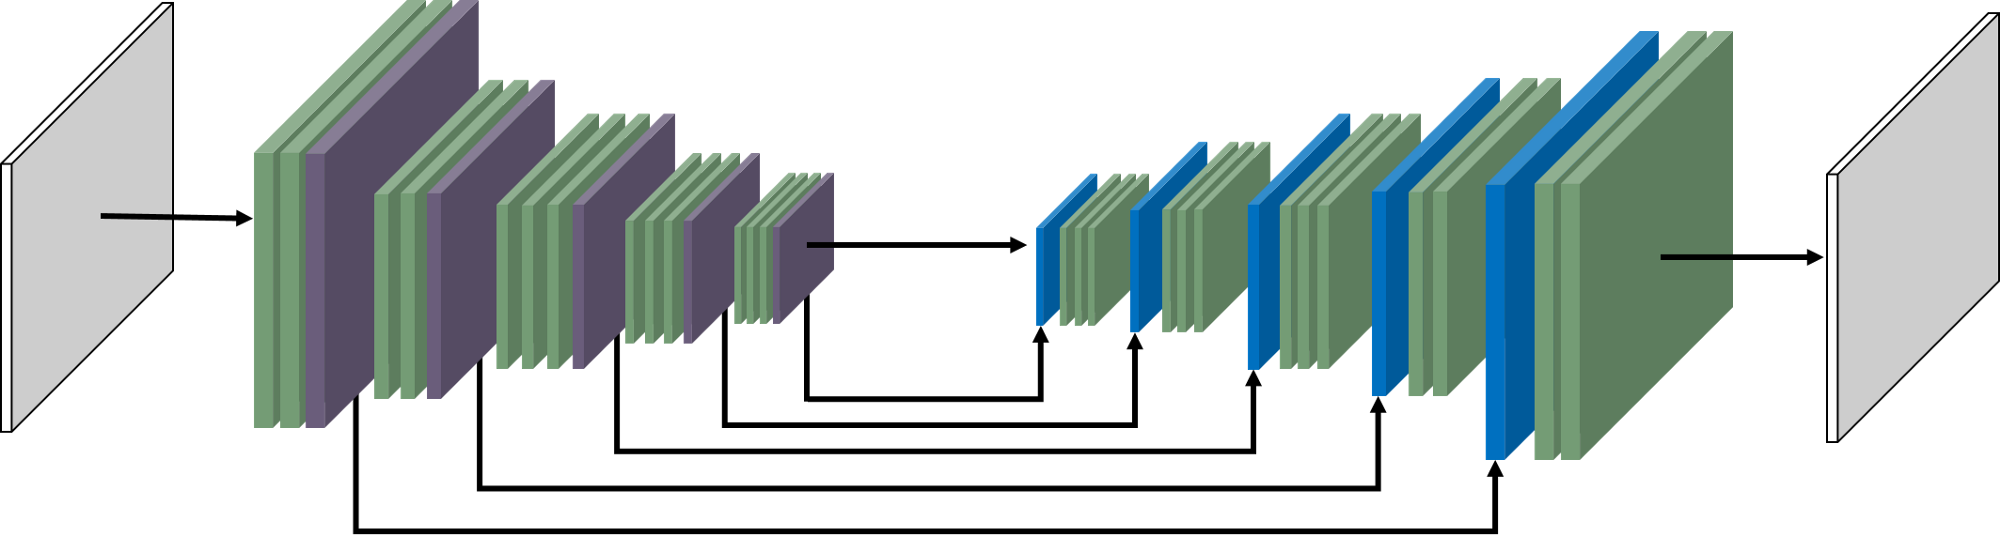
\includegraphics[width=\textwidth]{hourglass.png}
    \caption{Exemple d'architecture Hourglass}
\end{figure}


J'ai essayé de ne prédire que le centre de l'oeil à partir d'une image de l'oeil.
Pour obtenir des données de formation, j'ai utilisé le jeu de données de \href{http://cs.uef.fi/pupoint/}{crowdpupil}, qui consiste en $792$ images, chaque image étant étiquetée avec la position du centre de l'oeil.
Il existe deux méthodes pour essayer de prédire les points de repère du visage : essayer de trouver les coordonnées exactes $(x, y)$ par régression, ou essayer de reconstruire des cartes thermiques qui contiennent ces points de repère du visage.


J'ai choisi la deuxième option, et j'ai donc généré une carte thermique pour chaque image de l'oeil qui codait le centre de l'oeil.
J'ai mesuré une moyenne pour la distance entre le centre de la pupille et sa marge, et je l'ai utilisée comme ``variance'' pour une Distribution Gaussienne 2D, centrée dans l'oeil.

\begin{figure}[h]
    \centering
    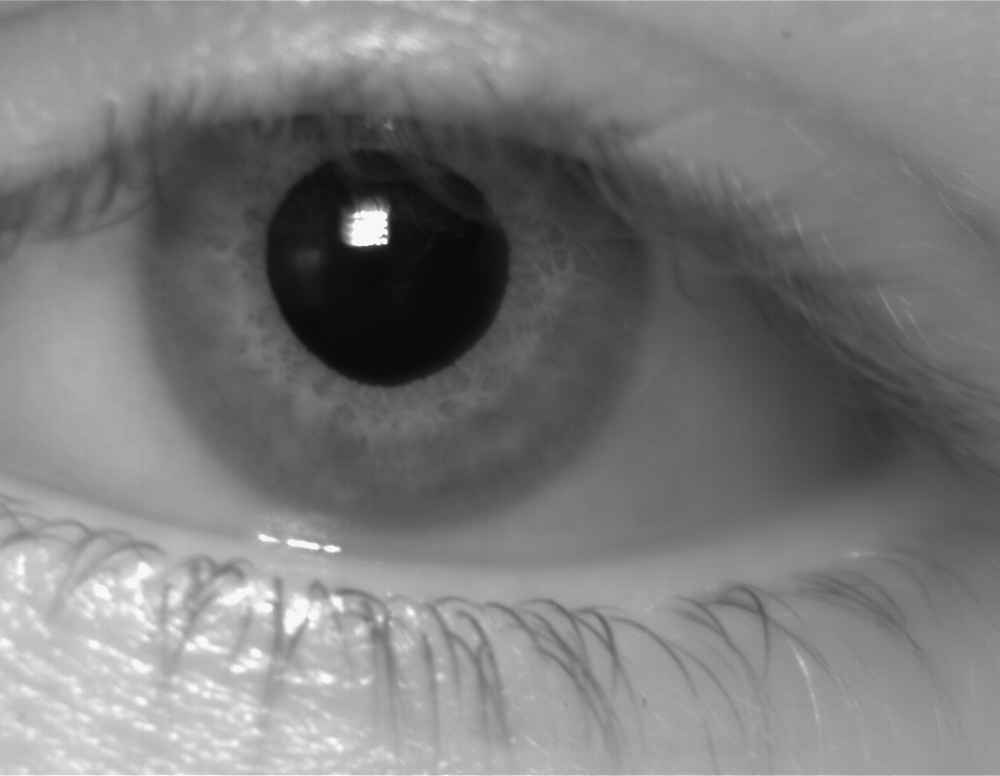
\includegraphics[width=0.32\textwidth]{Img_002_L_2.jpg}
    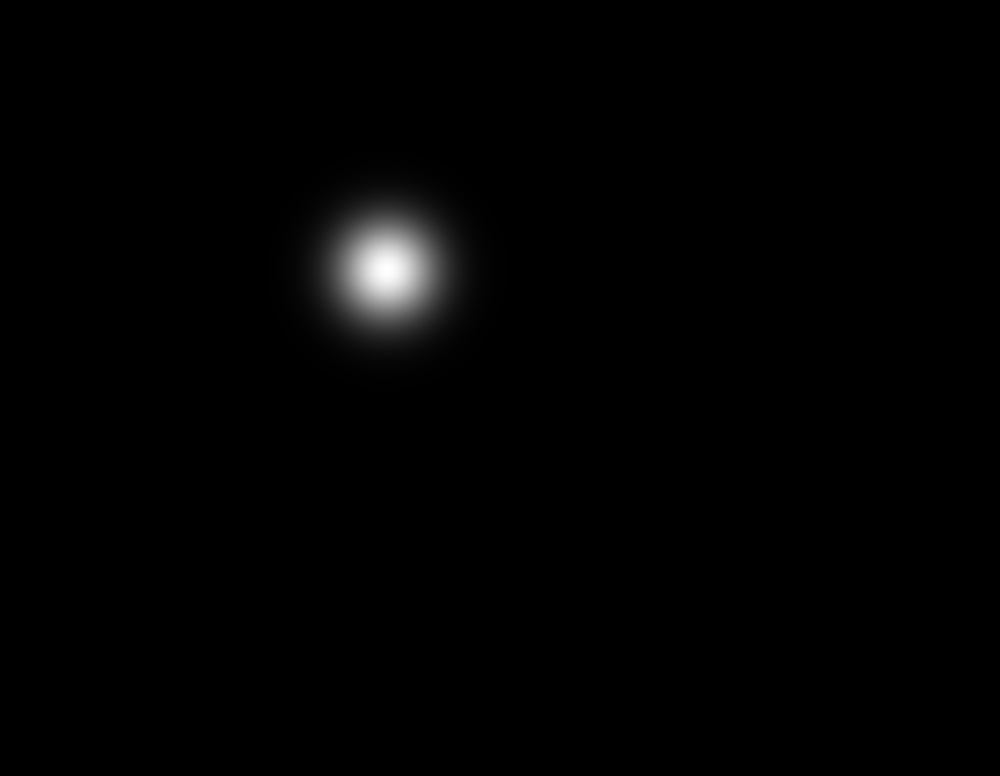
\includegraphics[width=0.32\textwidth]{h_Img_002_L_2.jpg}
    \caption{Centrul ochiului codificat printr-o hartă termografică}
\end{figure}

\clearpage


Après diverses expériences, j'ai découvert que je pouvais assez bien reconstruire les cartes thermiques en utilisant une \emph{architecture simplifiée} de CNN Hourglass :

\begin{lstlisting}[language=python]
class MyCNN(nn.Module):
    def __init__(self, input_size):
        super(MyCNN, self).__init__()
        ## eye image -> encoder -> decoder -> heatmap
        filters = [16, 32, 64, 128]
        # starting encoding
        self.layer1 = nn.Sequential(
            nn.Conv2d(1, filters[0], kernel_size=3, padding=2),
            nn.MaxPool2d(kernel_size=2, stride=2, padding=1),
            nn.ReLU(inplace=True),
            nn.BatchNorm2d(filters[0]),
            
            nn.Conv2d(filters[0], filters[1], kernel_size=2, padding=2),
            nn.MaxPool2d(kernel_size=2, stride=2, padding=1),
            nn.ReLU(inplace=True),
            nn.BatchNorm2d(filters[1]),
            
            nn.Conv2d(filters[1], filters[2], kernel_size=3, padding=2),
            nn.MaxPool2d(kernel_size=2, stride=2, padding=1),
            nn.ReLU(inplace=True),
            nn.BatchNorm2d(filters[2]),
            
            nn.Conv2d(filters[2], filters[3], kernel_size=2, padding=1),
            nn.MaxPool2d(kernel_size=2, stride=2, padding=1),
            nn.ReLU(inplace=True),
            nn.BatchNorm2d(filters[3]),
        )
        # encoding done, starting decoding
        self.layer2 = nn.Sequential(
            nn.Upsample(size=(28, 35), mode='bilinear'),
            nn.ConvTranspose2d(filters[3], filters[2], kernel_size=2, stride=1, padding=1),
            nn.ReLU(inplace=True),
            nn.BatchNorm2d(filters[2]),
            
            nn.Upsample(size=(54, 68), mode='bilinear'),
            nn.ConvTranspose2d(filters[2], filters[1], kernel_size=3, stride=1, padding=2),
            nn.ReLU(inplace=True),
            nn.BatchNorm2d(filters[1]),
            
            nn.Upsample(size=(104, 132), mode='bilinear'),
            nn.ConvTranspose2d(filters[1], filters[0], kernel_size=2, stride=1, padding=2),
            nn.ReLU(inplace=True),
            nn.BatchNorm2d(filters[0]),
        
            nn.Upsample(size=(202, 258), mode='bilinear'),
            nn.ConvTranspose2d(filters[0], 1, kernel_size=3, stride=1, padding=2),
            nn.ReLU(inplace=True),
            nn.BatchNorm2d(1),
        )
\end{lstlisting}


J'ai formé le réseau pendant $12$ époques, en utilisant comme optimiseur Adam et comme score MSE.
Pour la dernière époque, la moyenne des erreurs sur l'ensemble des données de test (environ $20\%$ du total des données) était de $8,425983$.
Voici le réseau essayant de reconstruire les cartes thermiques à partir des images des yeux :

\begin{figure}[h]
    \centering
    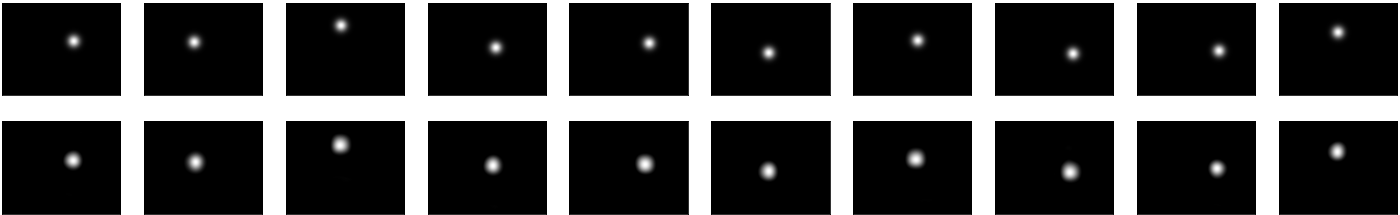
\includegraphics[width=\textwidth]{heatmap_predictions.png}
    \caption{Reconstruirea hărților termografice. Prima linie reprezintă adevărul de bază, iar a doua linie rezultatele modelului antrenat}
\end{figure}


Cependant, l'utilisation du réseau sur des images de mes propres yeux n'a pas vraiment donné de bons résultats.
L'une des raisons est que la qualité de ma webcam n'est pas très bonne et que les images des yeux extraites étaient très bruyantes.
% However, using the network on images of my own eyes didn't really give good results.
% One of the reasons is that my webcam's quality isn't very good and the images of the extracted eyes were very noisy.

\begin{figure}[h]
    \centering
    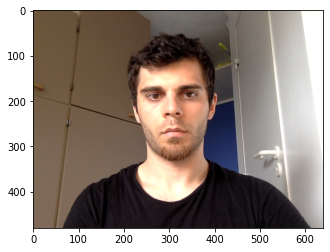
\includegraphics[width=0.32\textwidth]{heatmap_test.png}
    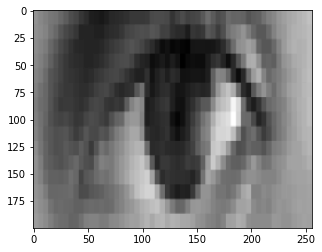
\includegraphics[width=0.32\textwidth]{heatmap_eye.png}
    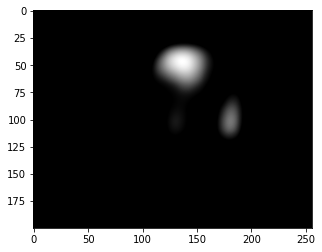
\includegraphics[width=0.32\textwidth]{heatmap_result.png}
    \caption{Tester le réseau Hourglass sur des images de moi-même}
\end{figure}